\documentclass{article}
\usepackage{pgffor}
\usepackage{tikz}
\usepackage{xfp}
\usepackage{mathtools}
\usetikzlibrary{calc, shapes.multipart,chains,arrows,positioning}

\tikzset{strela/.style={thick, ->, >=stealth}}

\newcommand\x{9}
\newcommand\y{3}
\newcommand\m{5}

\begin{document}
    
    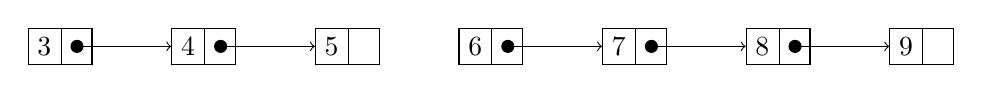
\begin{tikzpicture}[ar/.style={*->,shorten <=-.28cm},list/.style={rectangle split, rectangle split parts=2, draw, rectangle split horizontal}, start chain=going right]
        
                    
            \foreach \i in {3,...,\the\numexpr\x}{
              \ifnum\i=6
                \node[list,on chain] (\the\numexpr\i) {\i};
              \else
                \node[list,on chain,join=by ar] (\the\numexpr\i) {\i};         
              \fi
            }  
        
        
    \end{tikzpicture}


\end{document}